\chapter{Solving the Cross-Subject Parcel Matching Problem using Optimal Transport}
%
\section{Overview}
Matching structural parcels across different subjects is an open problem in neuroscience.
Even when produced by the same technique, parcellations tend to differ in the number, shape, and spatial localization of parcels across subjects.
In this work, we propose a parcel matching method based on Optimal Transport.
We test its performance by matching parcels of the Desikan atlas, parcels based on a functional criteria and structural parcels.
We compare our technique against three other ways to match parcels which are based on the Euclidean distance, the cosine similarity, and the Kullback-Leibler divergence.
Our results show that our method achieves the highest number of correct matches.

\section{Introduction}
Brain organization displays high variability across individuals and species. Studying brain connectivity therefore faces the challenge of locating homogeneous regions while accounting for this variability. Different techniques have been proposed to parcellate the brain based on its structural connectivity. However, matching the resulting parcels across different subjects is still an open problem in neuroscience. Even when produced by the same technique, parcellations tend to differ in the number, shape, and spatial localization of parcels across subjects \cite{Jbabdi2013}. Current theories hold that long-range structural connectivity, namely, extrinsic connectivity, is strongly related to brain function \cite{Passingham2002}. Therefore, being able to match parcels with similar connectivity across subjects can help to understand brain function while also enabling the comparisons of cortical areas across different species \cite{Mars2018}.
% Sam: In MIC, one of the interest is image segmentation/registration. Can you make a very clear link to this?

Most of the current methods to match parcels across subjects are strongly linked to the technique used to create them. For example, Moreno-Dominguez et al. \cite{Moreno-Dominguez2014} seek correspondences between dendrograms created by means of Hierarchical Clustering. Parisot et al. \cite{Paristot2015} impose the consistence of parcels across subjects while creating the parcellation. In recent works Mars et al. propose to use the Manhattan distance, cosine similarity \cite{Mars2016} or the Kullback–Leibler (KL) divergence \cite{Mars2018} to compare and match connectivity fingerprints, successfully identifying common areas across humans and primates.

In this work, we propose to match parcels based on their extrinsic connectivity fingerprint using Optimal Transportation theory. Optimal Transport (OT) is a technique that seeks the optimal way to transport mass between probability distributions. While KL divergence computes the difference between two distributions, OT computes a matching between them. In particular, our method adopts a discrete regularized version of Optimal Transport (OT), which has been presented in Gayraud et al.~\cite{nathalie} and Courty et al.~\cite{remi} as a solution to the domain adaptation problem.

\begin{figure*}[t!]
\centering
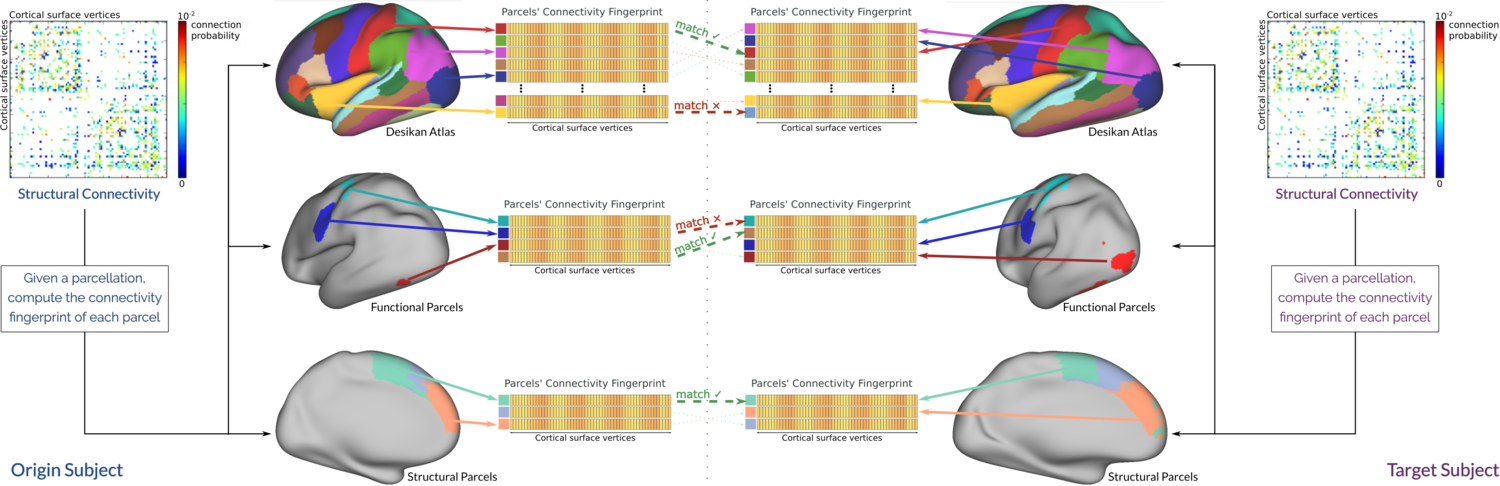
\includegraphics[width=1\textwidth]{6.matching/img/method}
\caption{From the cortico-cortical structural connectivity matrix of a subject, we can estimate the connectivity fingerprints of each parcel in three different types of parcellations. For each parcellation we compute the amount of correct matches (green lines) that each matching technique produces.}
\label{fig:method}
\end{figure*}

We validate our method with four different experiments. In the first experiment, we test the feasibility of our method by generating parcels with synthetic connectivity fingerprints and matching them. In the second one, we show that our technique is able to match parcels of the same atlas across subjects. We use the anatomical atlas of Desikan \cite{Desikan2006} as its parcels have high spatial coherence and consistent connectivity profiles across subjects \cite{DeReus2013}. Finally, we show the capacity of our method to match parcels generated with the same criteria but have some spatial cross-subject variability. We assess this for two different situations. In the first one, we derive the parcels from functional activations~\cite{Barch2013}. We use responses to motor and visual stimuli since they have been shown to be strongly related to structural connectivity~\cite{Osher2016, Penfield1954}. In the second one, we divide the Lateral Occipital Gyrus in 3 parcels using a structurally-based parcellation technique  \cite{Gallardo2017a}. We use the Lateral Occipital Gyrus since it has been shown to have a consistent parcellation across subjects \cite{ThiebautdeSchotten2016, Gallardo2017a}. The outline of the last three experiments can be seen in Figure~\ref{fig:method}.

In each experiment, we compare our technique against three other ways to match parcels based on the Euclidean distance; the cosine similarity; and the Kullback-Leibler divergence. Our results on real data show that our method based on OT always achieves the highest number of correct matches.


\section{Methods}

Given two subjects with their respective parcellations, we compute their parcel matching by considering one as the origin and the other one as target. 
More formally, let $X^a = \{x^a_i\}_{i=1}^{N_a}$, $x^a_i \in \Omega^a \subset \mathbb{R}^n$ be an origin dataset where $N_a$ denotes the number of parcels; $x^a_i$ is the extrinsic connectivity fingerprint of parcel $i$; and $n$ denotes its dimension. We wish to recover a matching between $X^a$ and a target dataset ${X^b = \{x^b_i\}_{i=1}^{N_b}}$, $x^b_i \in \Omega^b \subset \mathbb{R}^n$.
% Sam: What is an extrinsinc connectivity fingerprint? Where does it come from?
% You talk about extrinsic connectivity but you don't use the word fingerprint in the intro.
% Maybe start this section with a word on diffusion, tractography, and the inputs you need.

% Sam: How do you represent a matching? A permutation matrix? Nath: originaly yes, but it didn't fit. Is the structure that represents the matching important? Sam: well, this paragraph sounds like a problem statement, but at the end I still don't now what you are trying to find.

In this section, we start by formulating our  regularized discrete OT-based method and proceed by presenting three ways of computing this matching that are based on the Euclidean distance; the cosine similarity; and the KL-divergence.

\subsection{Discrete Regularized Optimal Transport}

Optimal Transport (OT) theory boils down to finding the optimal way to  transport or redistribute mass from one probability distribution to another with respect to some cost function.
In this work, since the datasets $X^a$ and $X^b$ are discrete datasets, we use their empirical probability distributions and apply the discrete formulation of OT~\cite{nathalie,remi} to solve the parcel matching problem. A simplified example of how our method proceeds is presented in Figure~\ref{fig:otprob}.

Assume that $X^a$ and $X^b$ follow probability distributions $p_a(x^a)$ and $p_b(x^b)$, respectively. We suppose that $X^a$ has undergone a transformation $\mathbf{T}:\Omega^a \rightarrow \Omega^b$, such that $p_b(\mathbf{T}(x^a)) = p_b(x^b)$. We wish to recover $\mathbf{T}$ and use it to match the parcels of $X^a$ and $X^b$. Using discrete regularized OT we compute a transport plan $\gamma_0$ between these two probability distributions. This transport plan is a doubly stochastic matrix which minimizes a certain transportation cost $C$ over the vectors of $X^a$ and $X^b$. In other words, it defines the optimal exchange of mass between the two probability distributions. We use $\gamma_0$ to compute an estimation $\hat{\mathbf{T}}$ by selecting the pairs of vectors, i.e., parcels that exchange the most mass. 
% Sam: I think this requires a bit more detail. What do you mean by a transport plan? I am guessing its
% related to T. Then, how does that transport plan give you a matching 
%Nath: Hopefully it is better explained now

Since $p_a(x^a)$ and $p_b(x^b)$ are not known, we use the corresponding empirical distributions $\mu_a = \sum_{i=1}^{N^a} p_i^a\delta_{x^a_i}$ and $\mu_b =\sum_{j=1}^{N^b} p_j^b\delta_{x^b_j}$ instead, where $p_i^a$ and $p_j^b$ are the probability masses associated to each sample. However, given that the dimension of our data depends on the number of vertices in the cortical mesh, the curse of dimensionality makes the estimation of $\mu_a$ and $\mu_b$ intrinsically difficult. We therefore simply assume a uniform probability distribution over all vectors, $p_i^a = \frac{1}{N^a}$ and $p_j^b = \frac{1}{N^b}$. We compute the transport plan $\gamma_0$ such that, if
% Sam: here the transport plan is gamma? How is it related to T?
% Explained in the intro and later

\begin{equation}
{\mathcal{B} = \big\{ \gamma \in (\mathbb{R}^+)^{N_a\times N_b} \mid \gamma \mathbf{1}_{N_b} = \frac{1}{N^a}\mathbf{1}_{N_a}, \gamma^{\mathbf{T}} \mathbf{1}_{N_a} = \frac{1}{N^b}\mathbf{1}_{N_b}  \big\}}
\end{equation}
denotes the set of all doubly stochastic matrices whose marginals are the probability measures $\mu_a$ and $\mu_b$, where $\mathbf{1}_N$ is an $N$-dimensional vector of ones, then $\gamma_0 \in \mathcal{B}$ is the output of the following minimization problem.
% Sam: Don't add a new line after equations or latex adds a new paragraph indentation.

\begin{figure*}[t!]
    \centering
    \begin{subfigure}[t]{0.32\textwidth}
        \centering
        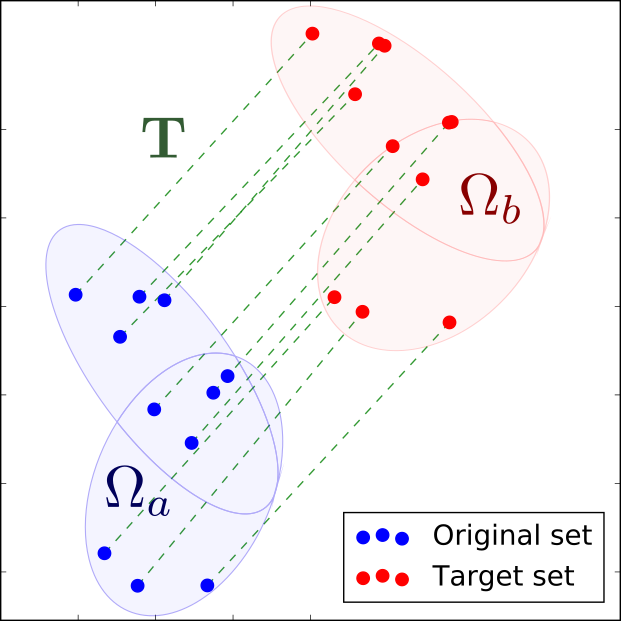
\includegraphics[height=1.4in]{6.matching/img/one}
        \caption{{\scriptsize Original \& target datasets}}
        \label{fig:otprob_a}
    \end{subfigure}%
    ~ 
    \begin{subfigure}[t]{0.32\textwidth}
        \centering
        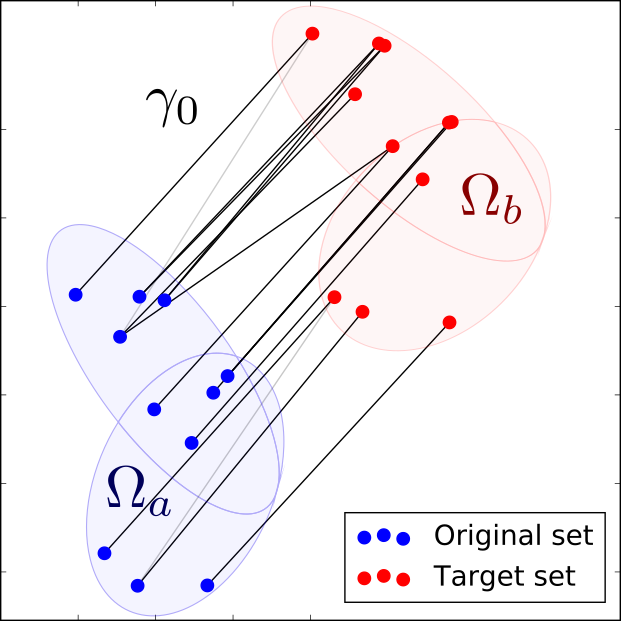
\includegraphics[height=1.4in]{6.matching/img/two}
        \caption{{\scriptsize Computed transport plan}}
        \label{fig:otprob_b}
    \end{subfigure}
    ~
    \begin{subfigure}[t]{0.32\textwidth}
        \centering
        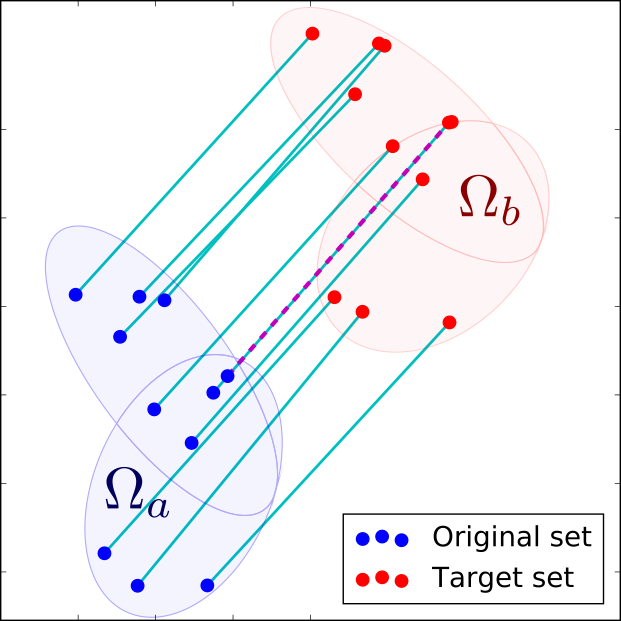
\includegraphics[height=1.4in]{6.matching/img/three}
        \caption{{\scriptsize Matching}}
        \label{fig:otprob_c}
    \end{subfigure}
    \caption{{\footnotesize A 2-d example of using OT to compute the matching between two different datasets. On the left we show the original and target datasets. The real matchings are displayed as green dashed edges. In the middle, the edge densities represent the values of the computed coupling $\gamma_0$, which denote the amount of mass that is exchanged between vectors $x_i^a$ and $x_j^b$. On the right, we see the recovered matching. The blue edges represent the correct matchings, while the red dotted edges represent the incorrect ones.}}
    \label{fig:otprob}
\end{figure*}

\begin{equation}
\gamma_0 = \argmin_{\gamma \in \mathcal{B}} \textnormal{~} \langle \gamma,C \rangle_F + \lambda \sum_{i,j} \gamma(i,j) \textnormal{~log~} \gamma(i,j)
\end{equation}
The matrix $C$, where $C(i,j) = \Vert x^a_i - x^b_j \Vert^2_2$, represents the cost of moving probability mass from location $x^a_j$ to location $x^b_i$, in terms of their squared Euclidean distance. The rightmost term is a regularization term based on the negative entropy of $\gamma$ allows us to solve this optimization problem using the Sinkhorn-Knopp algorithm~\cite{cuturi_sh} which improves the computation time.

Matrix $\gamma_0$ contains information about the exchange of probability mass between the vectors of $X^a$ and $X^b$. By construction, this exchange depends on the selected cost function. The choice of the squared euclidean distance is motivated both by the fact that it renders the optimization problem convex and because it will allow the parcels to be matched according to the vicinity of their feature vectors. Hence, the origin feature vectors will distribute their corresponding probability mass to the target feature vectors that are closest to them. Consequently, we define $\hat{\mathbf{T}}:\Omega^a \rightarrow \Omega^b$ as $\hat{\mathbf{T}}(x^a_i) = x^b_{\hat{j}}$ where $\hat{j} = \argmax_{j} \gamma_0(i,j)$. Therefore, $i$ will be matched to the parcel $\hat{j}$ that it sent the most mass to.

\subsection{Matching Parcels Based on Dissimilarity Between Features}
\label{sec:others}

% We define the three measures that we compare against our method. 
Let $d(x^a_i,x^b_j)$ be some dissimilarity measure between the elements of $X^a$ and $X^b$. Then, we say that parcel $i$ matches parcel $j$ if $\argmin_k d(x^a_i,x^b_k) = j$. We compare three dissimilarity measures against our method.
% ${d_e(x^a_i,x^b_j) = \lVert x^a_i - x^b_j \rVert_2}$, 
% ${d_c(x^a_i,x^b_j) =  1 - \{x^a_i\cdot x^b_j/\lVert x^a_i\rVert_2 \lVert x^b_j \rVert_2\}}$, and $d_{KL}(x^a_i,x^b_j) = \sum_{l=1}^d \tilde{x}^a_i(l) \log\{\tilde{x}^a_i(l)/\tilde{x}^b_j(l)\}$.
% \begin{equation*}
% \displaystyle
% d_e(x^a_i,x^b_j) = \lVert x^a_i - x^b_j \rVert_2
% \textnormal{,~~}
% d_c(x^a_i,x^b_j) =  1 - \frac{x^a_i\cdot x^b_j}{\lVert x^a_i\rVert_2 \lVert x^b_j \rVert_2}
% \textnormal{,~~and}
% \end{equation*}
% \begin{equation*}
% d_{KL}(x^a_i,x^b_j) = \sum_{l=1}^d \tilde{x}^a_i(l) \log\frac{\tilde{x}^a_i(l)}{\tilde{x}^b_j(l)}.
% \end{equation*}
First, we use the Euclidean distance, which  can be interpreted as matching the parcel $i$ to the parcel $j$ whose feature vector $x^b_j$ is the closest to $x^a_i$.
Then, we use the cosine similarity, which is minimized when two feature vectors are colinear. 
Lastly, we use the Kullback-Leibler divergence, which measures the difference between two probability distributions in terms of their relative entropy. Note that we need to convert our vectors into probability vectors in order to evaluate $d_{KL}$. 

% We therefore normalize each feature vector $x$ such that $\tilde{x} = \frac{x}{\rVert x \lVert_\infty}$, thus $\sum_{l=1}^d \tilde{x}(l) = 1$, where $\tilde{x}(l)$ is the $l$-th coordinate of $\tilde{x}$.

\section{Experiments and Results}

\subsection{Data and Preprocessing}
\label{sec:fingerprint}
For this work we randomly selected 20 subjects from the S500 group of the Human Connectome Project (HCP), all preprocessed with the HCP minimum pipeline~\cite{Glasser2013}. Fiber orientation distributions functions where computed using spherical constrained deconvolution with a spherical harmonic order of 8. Probabilistic tractography was then performed using 1000 seeds per vertex of the cortical mesh provided with the HCP data. For each subject, we computed a connectivity matrix by counting the number of streamlines that connect each pair of vertices of the cortical mesh. Each row in the matrix is a vertex connectivity vector, representing the probability that a connection exists between a surface vertex and the rest of the surface's vertices.
%\subsection{Computing a parcel's connectivity fingerprint}

Given a whole brain cortical parcellation, we compute the connectivity fingerprint of each parcel by averaging the connectivity fingerprint of its vertices. Because the mesh's vertices are coregistered across subjects~\cite{Glasser2013}, we are able to compare the connectivity fingerprints across subjects. The criterion to compute the parcel matching between two subjects is the similarity between connectivity fingerprints. That is, we match two parcels if they are connected to the rest of the brain in a similar manner. Due to the distance bias that occurs in tractography, a parcel tends to be highly connected to the vertices that compose it. To prevent the matching to be influenced by this bias, we disconnect each parcel from its own vertices.

%The main advantages of using this public data base are the following. First, each subject possess a dense mesh representing their cortical surface, which we use to create seed-points for tractography. Then, all the mesh's vertices are coregistered across subjects, a property that allows us to compare connectivity fingerprints across subjects. Additionally, each subject possess the Desikan Atlas~\cite{Desikan2006} parcellation already computed over their cortical mesh. Finally, for each cortical mesh, there are also different z-score maps representing the response to different stimuli obtained with functional MRI (fMRI)~\cite{Barch2013}. These z-score maps are used to compute a functional parcellation for each subject.
 
\subsection{Matching Parcels}
\label{sec:matching}
In this section we evaluate the performance of our method by comparing it to the methods presented in Section~\ref{sec:others}. For each experiment we compute parcel matchings between all possible pairs of connectivity matrices. To quantify the result of each technique, we compute the accuracy in terms of percentage of correctly matched parcels per pairwise matching.

\subsubsection{Matching parcels with synthetic fingerprints.}

In this first experiment, we test the feasibility of our method by generating parcels with synthetic connectivity fingerprints and matching them. We start by generating a connectivity matrix $M$ using probabilistic Constrained Spherical Deconvolution based tractography to use as ground truth. Our ground truth matrix is a square matrix that represents the connectivity between the 64 parcels of the Desikan atlas in one subject of the HCP dataset. Each coefficient $M(i,j) = \theta_{ij}$ is the parameter of a random variable that follows a Bernoulli distribution $X_{ij} ~ B(\theta_{ij})$. This variable $X_{ij}$ represents the probability of a connection existing between the parcels $i$ and $j$. 
Using $M$, we generate 20 synthetic matrices in such a way that the coefficients of each synthetic connectivity matrix are random variables that follow a binomial distribution $X(i,j) \sim B(p=M(i,j),n)$. 
By doing this we simulate doing tractography for various values of the number $n$ of particles. Figure~\ref{fig:synth} shows the performance of each method as a function of $n$.  


%To this date, no mathematical model has been found for the variability in extrinsic connectivity across subjects \cite{Paquette2016}. Therefore, we test our method in synthetic connectivity matrices created using 3 different methods. In each method, we simulate 20 connectivity matrices starting from a connectivity matrix $M \in R^{64 \times 64}$ between the parcels of the Desikan atlas, derived from probabilistic tractography. Each coefficient $M(i,j) = \theta_{ij}$ of the connectivity matrix is the parameters of a random variable that follows a Bernoulli distribution $X_{ij} ~ B(\theta_{ij})$. This variable $X_{ij}$ represents the probability of a connection existing between the parcel $i$ and $j$.

%In the second one, we follow a noise model similar to the one proposed by Paquette et al. \cite{Paquette2016} and generate synthetic connectivity matrices by adding multiplicative Gaussian noise on each row of $M$. In particular, the $i$-th row of each synthetic matrix $M'$ is equal to the inner product ${M'(i) = \langle M(i),X_i \rangle}$, where $X_i \sim \mathcal{N}(a_i\mathbf{1}_{64},\sigma)$, $\mathbf{1}_{64}$ is a $64$-dimensional vector of ones, and $a_i \sim \mathcal{N}(0,1)$.
%Finally, in the third experiment we generate synthetic connectivity matrices using the logistic random effects model presented in Gallardo et al. (2017). Each synthetic matrix $M'$ comes from the model $logit(M') = logit(M) + \Gamma$ where $\Gamma \sim N(0, \sigma \mathbf{I})$ is normally distributed noise and $\mathbf{I}$ is the identity matrix. That is, we add additive noise in the logit space.


%We show the performance of the first technique as a function of the number of realizations $n$, i.e., the number of simulated particles.
%The performance of the other two technique are displayed as a function of the standard deviation of the noise.

\begin{figure*}[t!]
    \centering
    \begin{subfigure}[t]{0.52\textwidth}
        \centering
        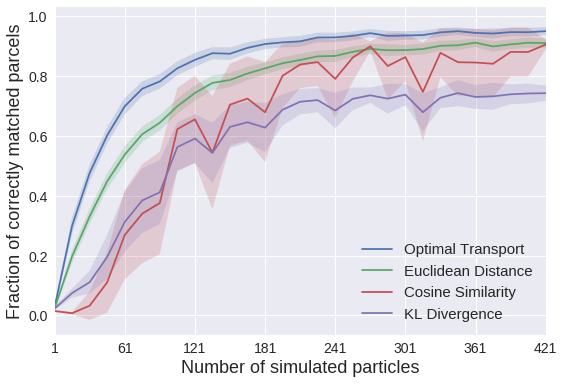
\includegraphics[height=1.7in]{6.matching/img/synthetic}
        \caption{{\scriptsize Synthetic data}}
        \label{fig:synth}
    \end{subfigure}%
    ~ 
    \begin{subfigure}[t]{0.52\textwidth}
        \centering
        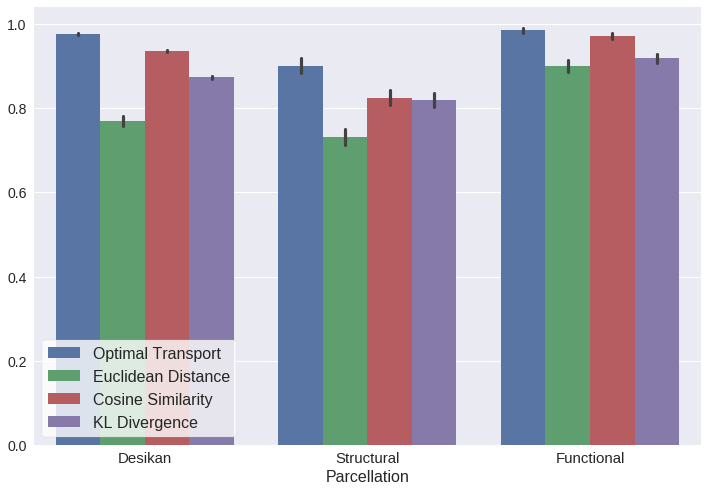
\includegraphics[height=1.7in]{6.matching/img/real}
        \caption{{\scriptsize Real data}}
        \label{fig:real}
    \end{subfigure}
    \caption{Proportion of parcels correctly matched by each method (see section~\ref{sec:others}) when matching: (a) synthetic connectivity fingerprints and (b) connectivity fingerprints of a cortical parcellation, for three different parcellations (as described in section~\ref{sec:matching}). OT always performs significantly better.}
    \label{fig:results}
\end{figure*}

\subsubsection{Matching parcels of the Desikan Atlas.}
For each subject, we compute the connectivity fingerprint of each parcel in their Desikan atlas as explained in Section \ref{sec:fingerprint}. When matching parcels across subjects, Figure~\ref{fig:real} shows that on average OT achieves an accuracy of 98\%$\pm$2\%, followed by cosine similarity (94\%$\pm$3\%), KL divergence (87\%$\pm$4\%), and finally Euclidean distance (77\%$\pm$11\%).

\subsubsection{Matching parcels created using functional criteria.}
Each subject in the HCP dataset possesses z-score maps representing responses to different stimuli obtained with functional MRI (fMRI)~\cite{Barch2013}. We derive parcels for each subject from the responses to motor (hand, foot and tongue movement) and visual stimuli (faces vs shape recognition). We do so by keeping only the vertices whose z-score is in the top 35\%.
Figure \ref{fig:real} shows that OT performs best with an average of 98\%$\pm$6\%. The cosine similarity, KL divergence, and Euclidean distance achieve average accuracies of 97\%$\pm$6\%, 92\%$\pm$10\%, and 90\%$\pm$13\% respectively.

\subsubsection{Matching parcels created using structural criteria.}
For each subject, we first mask their Lateral Occipital Gyrus using the Desikan atlas. Then, we divide it into 3 parcels using the structural based parcellation technique of Gallardo et al.~\cite{Gallardo2017a}. Once more, we can see on Figure \ref{fig:real} that optimal transport has the highest average accuracy, equal to 92\%$\pm$16\%. It is followed by the cosine similarity, the KL divergence, and the Euclidean distance, whose average accuracies equal 85\%$\pm$17\%, 84\%$\pm$17\%, and 75\%$\pm$17\%

\section{Discussion}
In this work we proposed a method to match parcels across subjects based on the connectivity fingerprint of a parcel. 

We tested our method with four different experiments. In the first experiment our technique correctly matched connectivity fingerprints created in a synthetic way. Specifically, each entry in a fingerprint was sampled from a Binomial distribution, whose parameter was chosen as the corresponding value of a ground truth connectivity matrix. This can be thought as a simulation of the process of tracking in tractography with different number of streamlines. 
%This choice of simulation was motivated by the results in Paquette et al. \cite{Paquette2006} which shows that neither additive nor multiplicative noise are adequate cross-subject variability models.

Our second experiment shows that we can correctly match parcels of the Desikan atlas across subjects with a 98\% of correct matches. The parcels of the Desikan atlas are known to have high spatial coherence and consistent connectivity profiles across subjects \cite{DeReus2013}. We therefore use this experiment as a reference point to benchmark our technique.
The last two experiments show that our technique can match parcels generated with a same criteria, even when they have some spatial variability across-subjects. The first experiment uses parcels created from the functional response to specific motor and visual stimuli, known to be strongly linked to functional connectivity \cite{Osher2016, Penfield1954}. The second one, parcels created from the structural parcellation of the Lateral Occipital Gyrus, a structure documented to have a consistent structural division \cite{ThiebautdeSchotten2016, Gallardo2017a}. 

It's important to notice that our technique achieved more than a 90\% of correct matches in every experiment with real data. Given that we used 20 subjects, this represents a total of 20x19=380 cross-subject matches. In the case of the Desikan atlas, which possesses 64 parcels, this translates into a total of 24320 matches, from which 98\% where correctly matched. Furthermore, when tested with a paired t-test to compare the number of correct matches, our method always performs significantly better than the other three ($p<10^{-256}$).

% The fact that OT transport performs well can also imply the kind of transformation which occurs between the connectivity fingerprints of two cross-subject parcellations. 

\section{Conclusion}
Matching structural parcels across different subjects is an open problem in neuroscience. In this work, we proposed a novel parcel matching method based on Optimal Transport. We tested its performance with four different experiments, always obtaining the highest number of correctly matched parcels, which is an improvement over the results of the currently used techniques. Our technique could have major implications in the study of brain connectivity and its relationship with brain function, allowing for the location of parcels with similar connectivity but not high spatial coherence. Also, it could help to understand the link between different brain atlases, and improve the  comparisons of cortical areas between higher primates.

 \section*{Acknowledgements}
This work has received funding from the European Research Council (ERC) under the Horizon 2020 research and innovation program (ERC Advanced Grant agreement No 694665 : CoBCoM), and from the ANR NeuroRef

%\bibliographystyle{splncsnat}
%\bibliography{bibtex}
